\documentclass[twocolumn]{article}
\setlength{\columnsep}{20pt}
%\usepackage{url}
%\usepackage{algorithmic}
\usepackage[a4paper]{geometry}
\usepackage{datetime}
\usepackage[font=small,labelfont=it]{caption}
\usepackage{graphicx}
% Use Times NR as font
\usepackage{lmodern}
\usepackage[T1]{fontenc}

\usepackage{float}

% Better tables
\usepackage{tabularx}
% to make beautiful tables
\usepackage{booktabs}

\usepackage{microtype}
\usepackage{amsmath}
\usepackage{subfigure}

% Letterspacing macros
\newcommand{\spacecaps}[1]{\textls[200]{\MakeUppercase{#1}}}
\newcommand{\spacesc}[1]{\textls[50]{\textsc{\MakeLowercase{#1}}}}

\title{\huge{\textbf{Study doc: embedding size experiment}}\\ \normalsize \Large{how does the size of the embedding space effect the triplet loss}}

\author{Fabian Gröger\\fabian.groeger@stud.hslu.ch}
\date{\today}

\begin{document}
\maketitle

\begin{abstract}
The experiment aims to show the effect of the size of the last dense layer from the embedding architecture, further called the \textbf{embedding size}.
\end{abstract}

\section{Introduction}
The size of the embedding space is essential for the performance, since choosing the wrong hyperparameter can lead to over- or underfitting of the model. The size defines how many dimensions the resulting embedding space has. Therefore if this parameter $e$ is selected to be too big, the model almost certainly overfits, because the model has many options to project the input data onto the embedding space. However, if $e$ is chosen to be too small, there is not enough room to project inputs in different regions. This experiment aims to search an optimal parameter for $e$.

\section{Hyperparameters}
The hyperparameters used for this experiment are shown in table \ref{tab:Hyperparameters}. The experiment will be conducted using a state of the art ResNet18 architecture on the DCASE dataset. The hyperparameters in section \textit{Feature representation} as well as the sample rate are the default ones proposed by the organisers of the DCASE challenge within the baseline project. The embedding size $e$ will be evaluated for four different values \texttt{[2, 16, 32, 64]}.

\begin{table}[H]
    \centering
    \caption{Hyperparameters used for the experiment}
	\label{tab:Hyperparameters}
    \begin{tabular}{l|l}
        \toprule
        \textbf{Hyperparameter} & \textbf{value} \\ 
        \midrule[1pt]
        Dataset & DCASE \\
        \hline
        Model & ResNet18 \\ 
        \hline
        Epochs & 20-50 \\ 
        \hline
        Batch size & 64 \\ 
        \hline
        Optimizer & Adam \\ 
        \hline
        Learning rate & 1e-5 \\
        \hline
        Margin & 1.0 \\
        \hline
        L2 regularisation amount & 0.1 \\
        \hline
        Embedding dimension & \textbf{[2, 16, 32, 64]} \\
        \hline
        Prefetch batches & Autotune (-1) \\ 
        \hline
        Random selection buffer & 32 \\ 
        \hline
        Shuffle dataset & True \\
        \hline
        Random seed & 1234 \\
        \midrule[1pt]
        \multicolumn{2}{l}{\textit{Multi threading}} \\
        \midrule[1pt]
        Number of generators & 16 \\ 
        \hline
        Number of parallel calls & 16 \\
        \midrule[1pt]
        \multicolumn{2}{l}{\textit{Audio sample}} \\
        \midrule[1pt]
        Sample rate & 16000 \\ 
        \hline
        Sample size & 10 \\
        \hline
        Sample tile size & 5 \\
        \hline
        Sample tile range & 5 \\
        \hline
        Convert to mono & True \\
        \midrule[1pt]
        \multicolumn{2}{l}{\textit{Feature representation}} \\
        \midrule[1pt]
        Feature extractor & LogMelExtractor \\ 
        \hline
        Frame length & 480 \\
        \hline
        Frame step & 160 \\
        \hline
        FFT size & 1024 \\
        \hline
        Number of Mel bins & 128 \\
        \hline
        Number of MFCC bins & 13 \\
        \bottomrule
    \end{tabular}
\end{table}

\begin{figure}[t]
\centering
    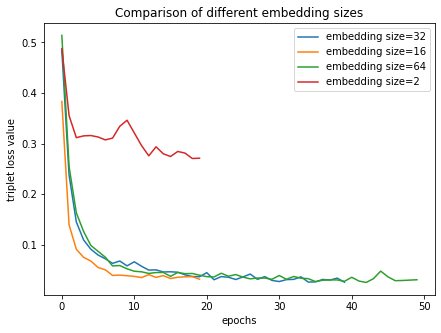
\includegraphics[width=\linewidth]{assets/plot_embedding_sizes.png}
    \caption{Plot of the triplet loss of the different embedding sizes}
    \label{fig:plot-embeddings-epochs}
\end{figure}

\section{Results}
Four models with the same hyperparameters, shown in table \ref{tab:Hyperparameters}, were trained for a different amount of epochs. The training was stopped when no more learning was observed. 

Comparing different embedding sizes is pretty hard since most of the metrics in the thesis focus on distances between embedding points. In higher dimensional embedding spaces, distances have a different scale and different meanings. This is especially true if small embedding sizes, such as \texttt{2}, and large sizes, such as \texttt{64}, are compared with each other. Therefore a simple classifier was trained on the resulting embedding spaces, and the metrics of the classifier was compared to find the optimal parameter. To further compare the embedding spaces, they were visualised using the Tensorboard Embedding Projector and manually compared with each other.

The figure \ref{fig:plot-embeddings-epochs} shows the different triplet loss values of the embedding sizes. The embedding size \texttt{2} has a significantly higher value than other embedding sizes, which shows that in the two-dimensional embedding space, it is a lot harder to project the data points apart from each other. Whereas in high dimensional embedding spaces, the model can easier build clusters.  

The plot further shows that the loss value of the embedding sizes \texttt{16, 32, 64} are relatively similar and are therefore further compared by examining their resulting embedding space. Which is shown in figure \ref{fig:embedding-space-16}, \ref{fig:embedding-space-32} and \ref{fig:embedding-space-64}. The result shows that there are vast differences in the embedding spaces, even though the triplet loss value is not that different. The embedding size of \texttt{16} shows only approximately four resulting clusters, which indicates a noisy embedding space where small classes are not well separated from each other. The embedding space of \texttt{32} and \texttt{64} show significant more resulting clusters and they result therefore in a better embedding space. However, it is to say that both embedding spaces further have more noise in it than the lower-dimensional space.

The line plot \ref{fig:classifier-f1} shows the resulting F1 score when a simple logistic classifier is trained on top of the resulting embedding space. Since the DCASE dataset is heavily unbalanced, the F1 score is compared. All of the classifiers are trained for 20 epochs using the same parameters as the one in table \ref{tab:Hyperparameters}. The figure \ref{fig:classifier-f1} shows that the F1 score of the embedding space \texttt{16} is the highest out of the three.

The line plot \ref{fig:classifier-loss} shows the sparse categorical cross-entropy loss value of the embedding spaces \texttt{16} and \texttt{64}.

\begin{figure}[t]
\centering
    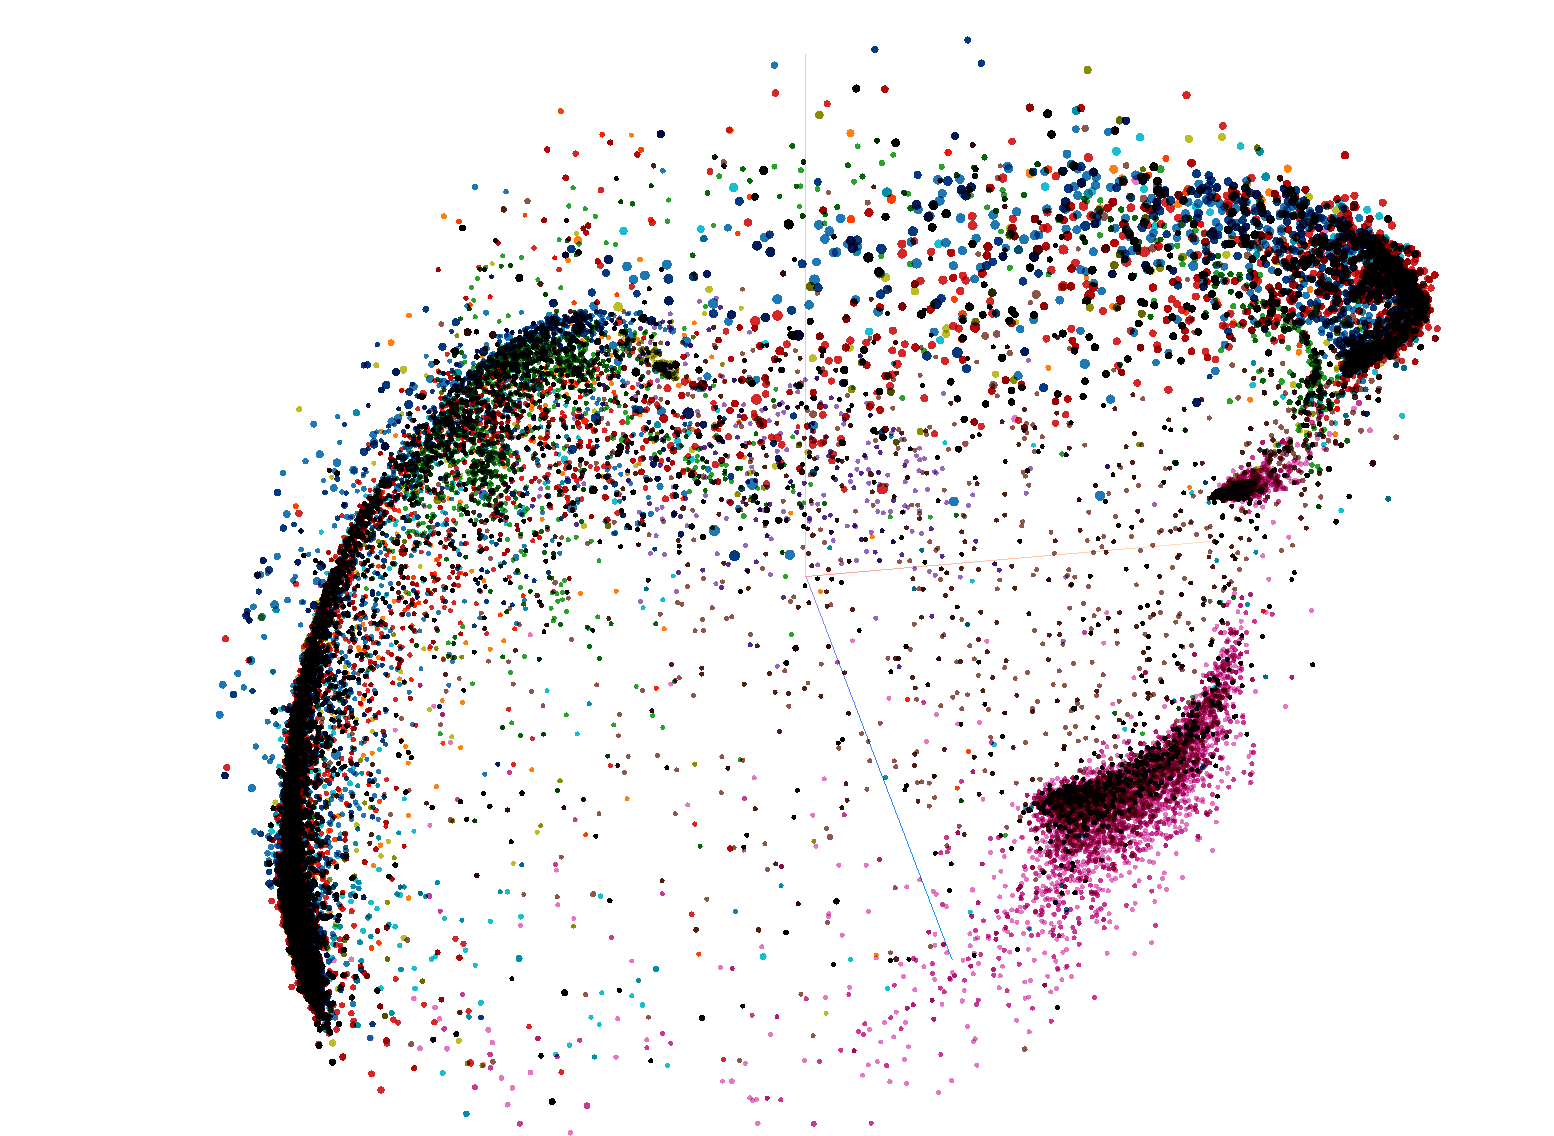
\includegraphics[width=\linewidth]{assets/embedding_space_16.png}
    \caption{Plot of the resulting embedding space of size 16}
    \label{fig:embedding-space-16}
\end{figure}

\begin{figure}[t]
\centering
    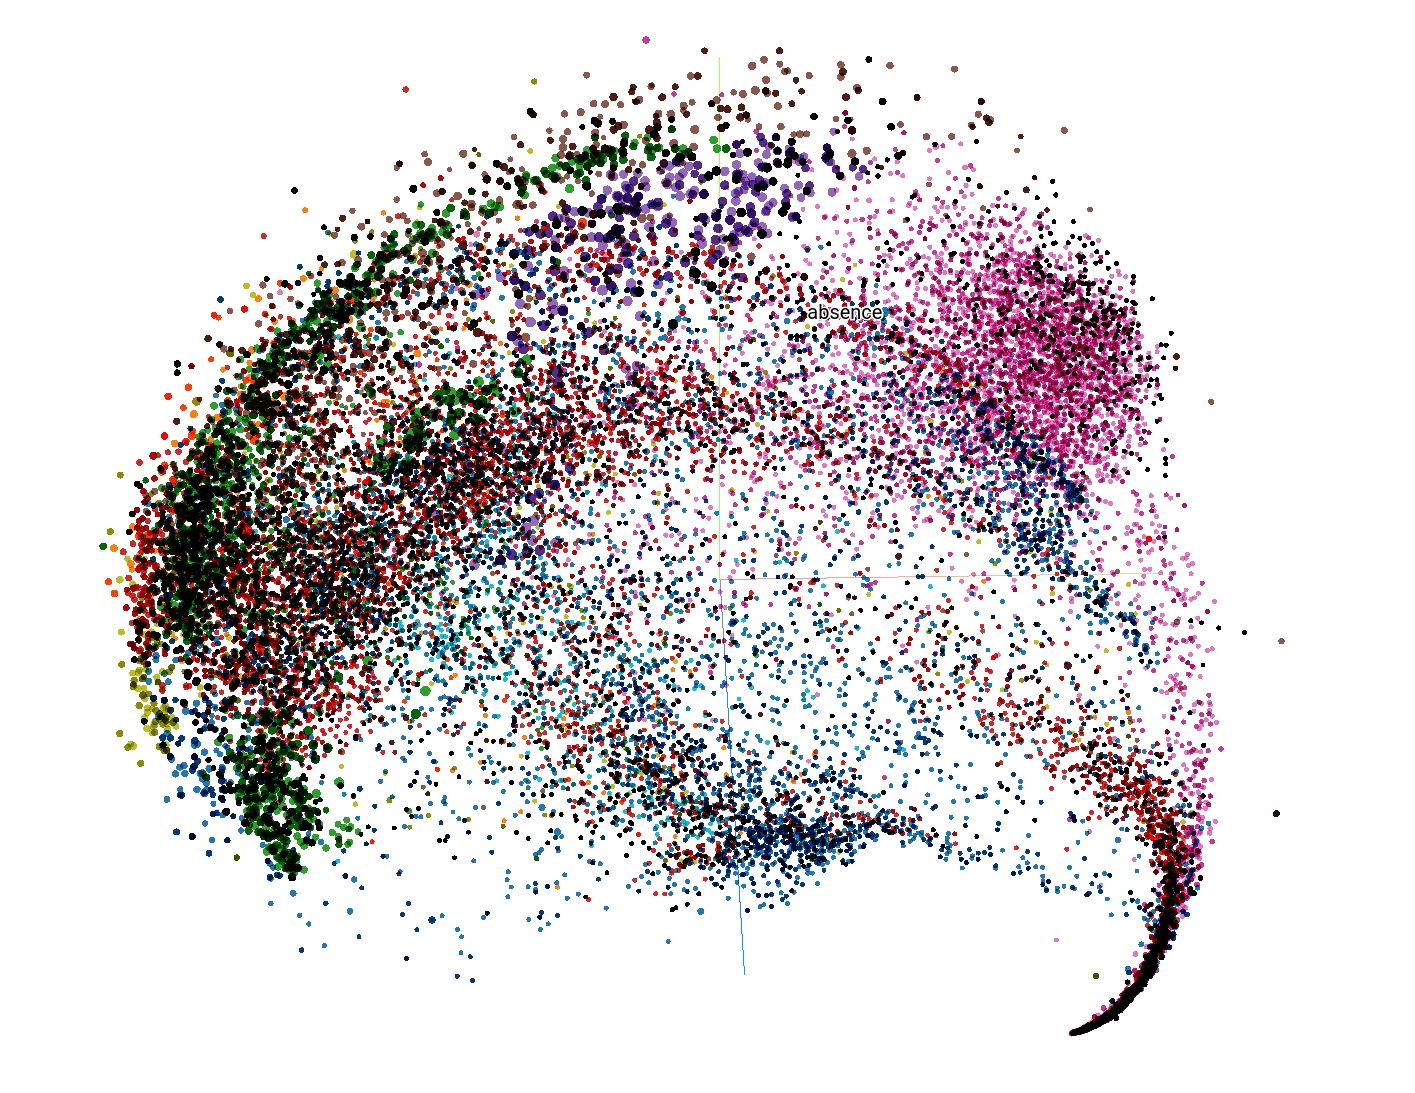
\includegraphics[width=\linewidth]{assets/embedding_space_32.png}
    \caption{Plot of the resulting embedding space of size 32}
    \label{fig:embedding-space-32}
\end{figure}

\begin{figure}[t]
\centering
    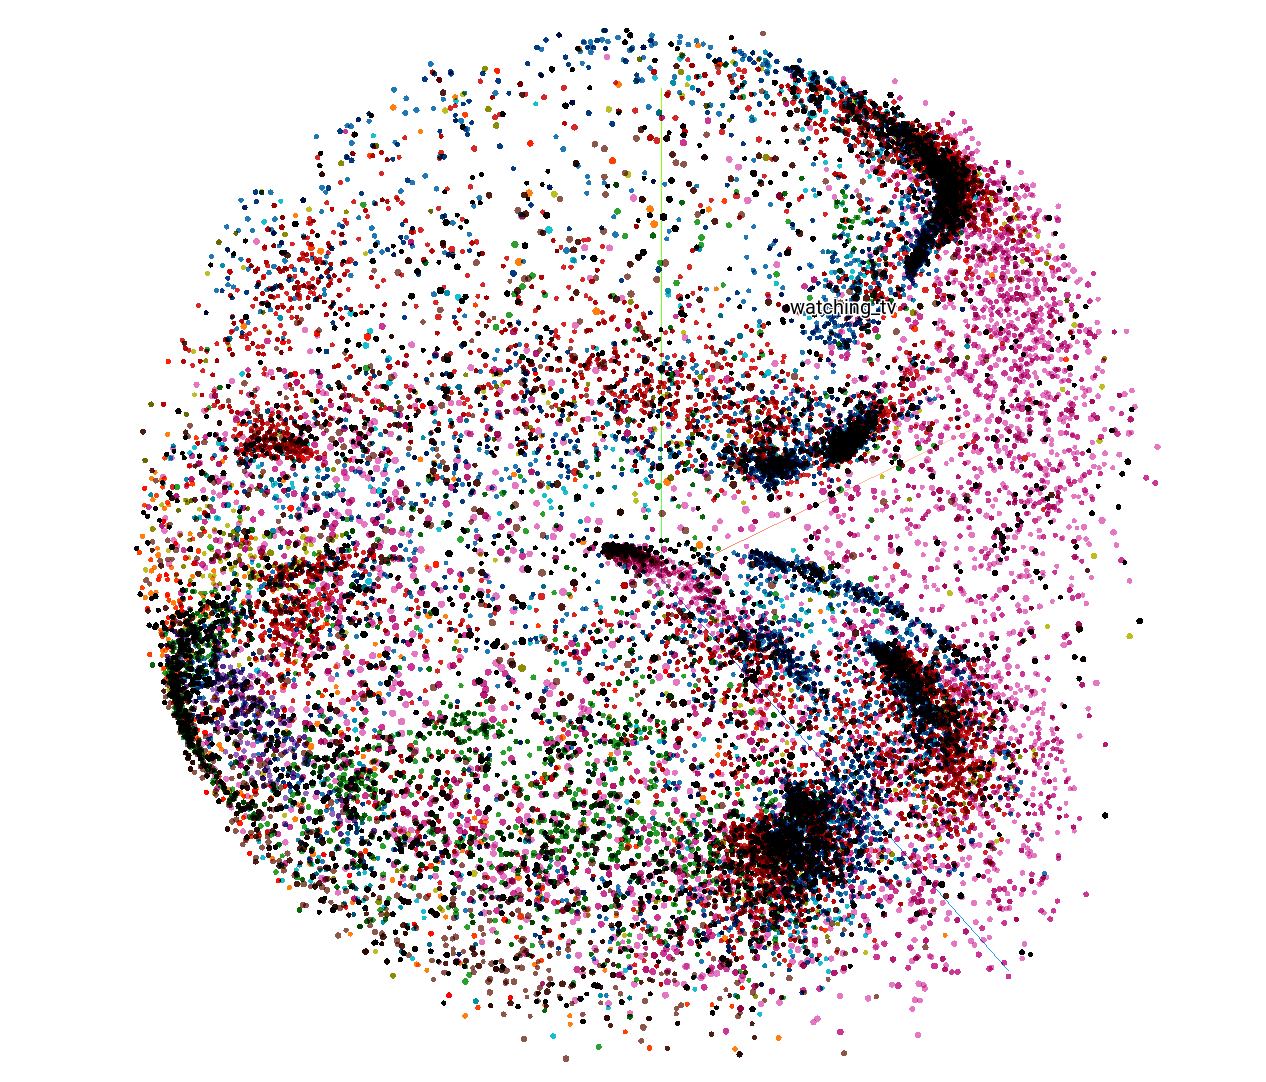
\includegraphics[width=\linewidth]{assets/embedding_space_64.png}
    \caption{Plot of the resulting embedding space of size 64}
    \label{fig:embedding-space-64}
\end{figure}

\begin{figure}[t]
\centering
    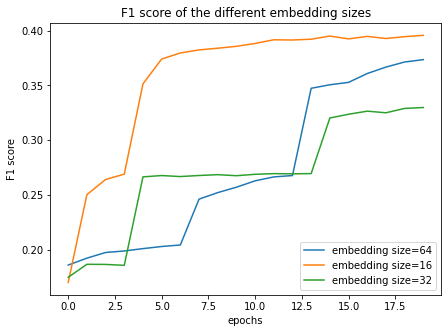
\includegraphics[width=\linewidth]{assets/classifier_f1.png}
    \caption{Line plot of the F1 score from the different classifiers trained on top of the resulting embedding spaces}
    \label{fig:classifier-f1}
\end{figure}

\begin{figure}[t]
\centering
    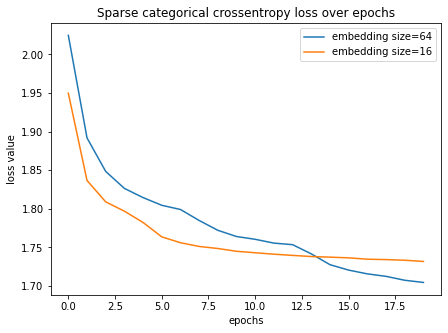
\includegraphics[width=\linewidth]{assets/classifier_loss.png}
    \caption{Line plot of the sparse categorical cross-entropy loss of the embedding size 16 and 64}
    \label{fig:classifier-loss}
\end{figure}

\section{Conclusion}
The figure \ref{fig:plot-embeddings-epochs} shows that the smallest embedding size can be omitted since it has the highest triplet loss value significantly. The other three embedding spaces have quite similar values and are, therefore, further compared. The trained classifier on top of the embedding space shows (figure \ref{fig:classifier-f1}) that the embedding size \texttt{32} can be omitted since it has a significantly lower score than the others. The figure \ref{fig:classifier-f1} shows, that the embedding size \texttt{16} has achieved the highest F1 score of approximately \texttt{0.39}. However, the figure \ref{fig:classifier-loss} shows that the loss value of the embedding size \texttt{16} converges, which indicates that the training process is finished and the classifier will not show any improvements when training longer. The embedding size \texttt{64} has a lower F1 score, but the loss value is still decreasing at the end of epoch 20, which indicates that the model can benefit from further training. Further training will increase the F1 score until it converges.

Because of this result, the optimal embedding size, out of the four, is \texttt{64}, since it has an optimal triplet loss value, a high enough F1 score and the loss value still decreases after 20 epochs of training the classifier.

\begin{figure}[t]
\centering
    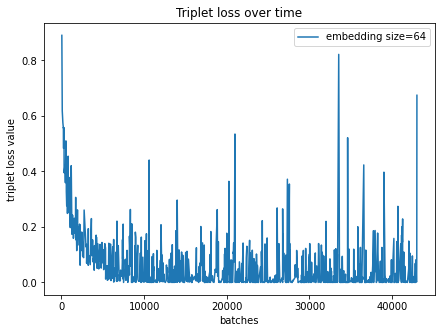
\includegraphics[width=\linewidth]{assets/plot_triplet_loss.png}
    \caption{Plot of the triplet loss of the embedding space 64}
    \label{fig:plot-triplet-64}
\end{figure}

\section{Next steps}
This experiment showed that changing the dimension of the embedding space results in significant different embedding spaces and therefore resulting clusters. The experiment should further be conducted for the music dataset because this parameter highly depends on the underlying structure of the data. 

For the next experiments, the embedding space size \texttt{64} is chosen. The embedding space should also be evaluated on significant higher spaces, such as \texttt{256} or \texttt{512}.

The experiment further showed another important conclusion, that the longer the embedding space is trained, the more the loss value oscillates which indicates that a learning rate decay should be used to reduce the learning rate over time (\ref{fig:plot-triplet-64}).

\end{document}